\begin{frame}{Resultados prelimiares}

    

    \begin{onlyenv}<1>
        Piezas mecánicas del perfilador
        \begin{columns}[c]
            \begin{column}{.6\textwidth}
                \begin{figure}
                    \centering
                    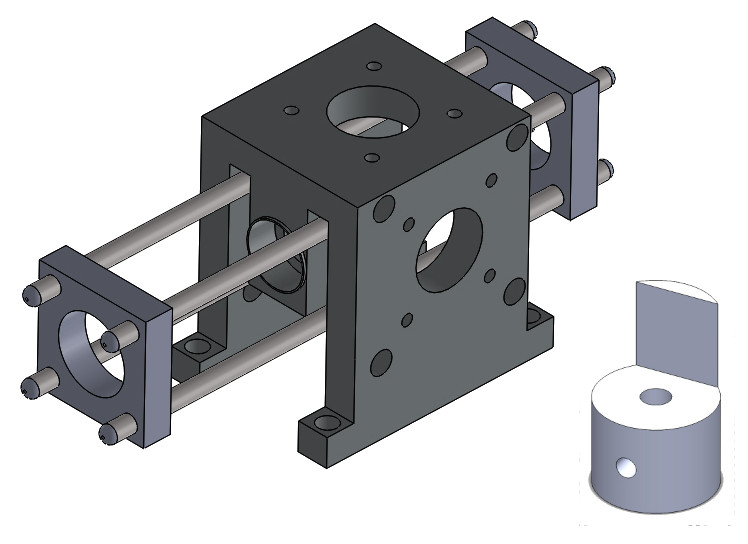
\includegraphics[width=\textwidth]{fig/perfilador/soporte_labo6}
                    \label{fig:pieza}
                \end{figure}
            \end{column}
            \begin{column}{0.4\textwidth}
                \centering
                \begin{figure}
                    \centering
                    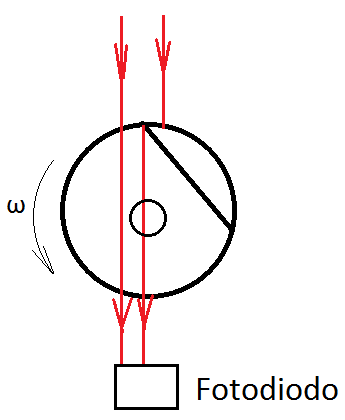
\includegraphics[width=0.8\textwidth]{fig/perfilador/corte_tambor}
                    \label{fig:pieza}
                \end{figure}
                Esquema de la perfilación del tambor
            \end{column}
        \end{columns}
    \end{onlyenv}

    \begin{onlyenv}<2>
        Electrónica de adquisición
        \begin{columns}[c]
            \begin{column}{0.3\textwidth}
                \begin{figure}
                    \centering
                    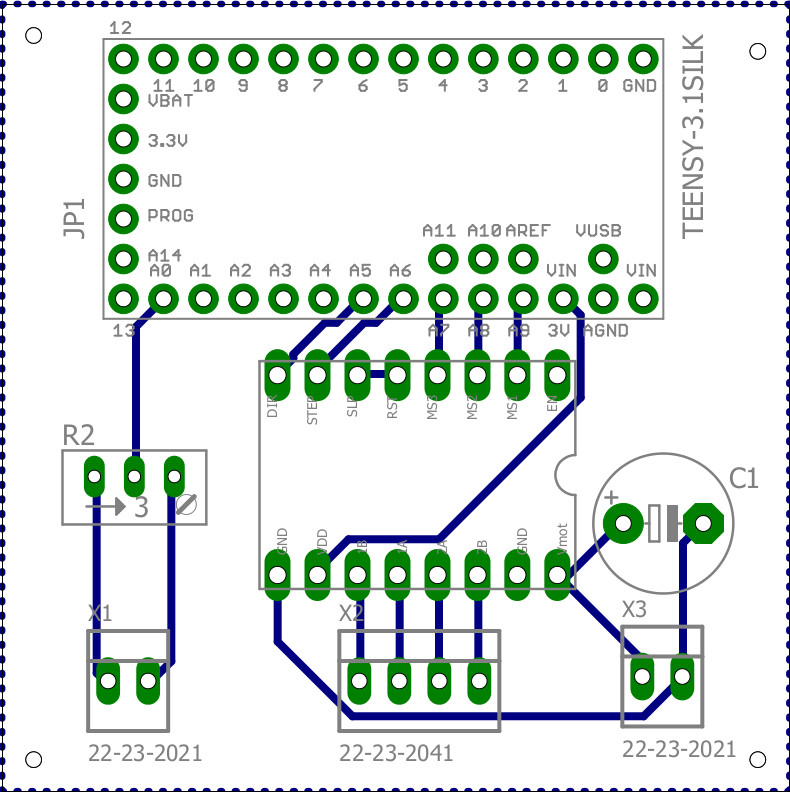
\includegraphics[width=\textwidth]{fig/circuito/circuito_labo6.jpg}
                    \label{fig:circuito}
                \end{figure}
            \end{column}
            \begin{column}{0.6\textwidth}
                \begin{itemize}
                    \item uC Teensy v3.2. CPU 96MHz, y 64KiB RAM. ADC 1Msps max. x10 Arduino Uno
                    \item Placa circuital de 5x5cm. Controla el motor y la adquisición al mismo tiempo. 
                    \item Ajuste de los datos por software. Hecho en Python
                    \item Máxima adquisición de 12 perfiles por segundo, limitación del uC/Software.
                \end{itemize}
            \end{column}
        \end{columns}
    \end{onlyenv}
    \end{frame}
    
    \begin{frame}{Mediciones prelimiares}
        \begin{onlyenv}<1>
        Mediciones a salida de colimador F220FC.
        \begin{columns}[c]
            \begin{column}{0.6\textwidth}
                 \begin{figure}
                    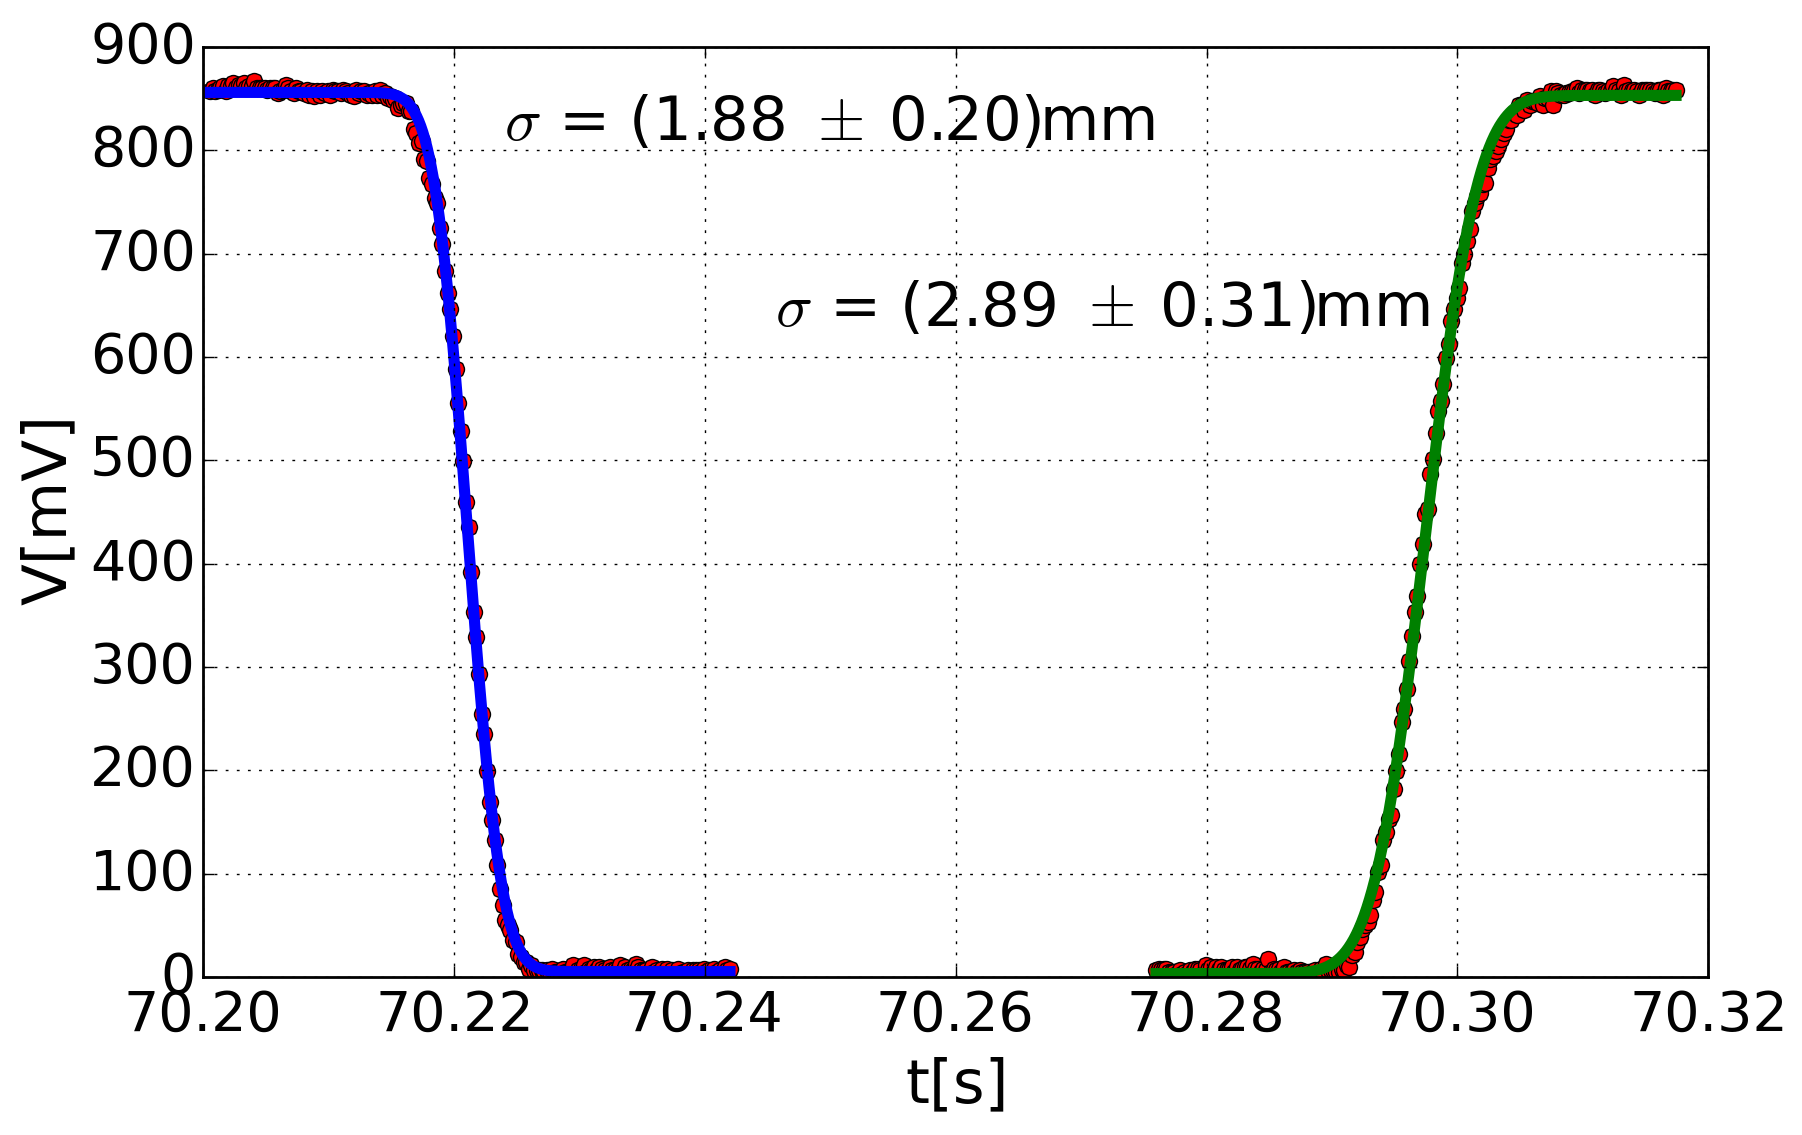
\includegraphics[width=\textwidth]{fig/perfilador/fit_data_labo6}
                    \label{fig:perfilador/fit_data_labo6}
                \end{figure} 
                
               
            \end{column}

            \begin{column}{0.4\textwidth}
                 \begin{figure}
                    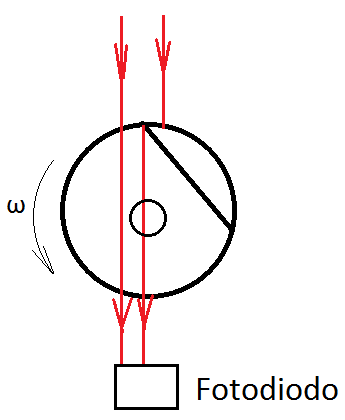
\includegraphics[width=0.4\textwidth]{fig/perfilador/corte_tambor}
                    \label{fig:perfilador/corte_tambor}
                \end{figure} 
                \begin{itemize}
                    \item Diferencia apreciable de tamaño de haz entre transiciones.
                    \item Es de origen mecánico, soporte no ajusta correctamente el motor
                \end{itemize}
            \end{column}
        \end{columns}
        
    \end{onlyenv}
    \begin{onlyenv}<2>
        
        \begin{columns}[c]
            \begin{column}{0.6\textwidth}
                \begin{figure}
                    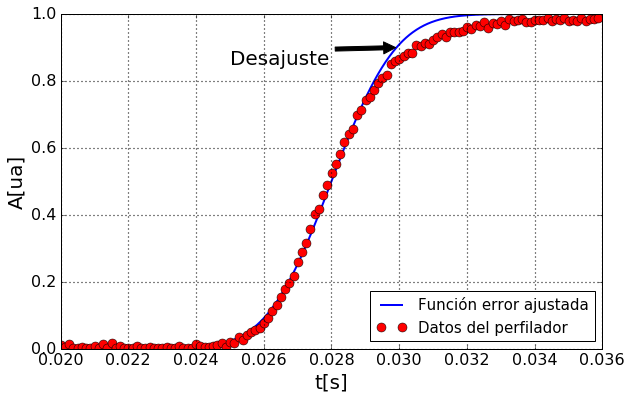
\includegraphics[width=\textwidth]{fig/perfilador/fit_data_labo6_anotado}
                    \label{fig:perfilador/fit_data_labo6_anotado}
                \end{figure} 
             \end{column}

            \begin{column}{0.4\textwidth}
                \begin{itemize}
                    \item Desajuste entre función error y datos al desobturar haz.
                    \item Fotodiodo con resistencia de carga enorme genera respuesta en frecuencia pobre.
                    \item Es necesario amplificar señal del fotodiodo
                \end{itemize}
            \end{column}
        \end{columns}
    \end{onlyenv}
\end{frame}
